\section{Stage}

\subsection{But}
%expliquer le sujet / les idées de départ :
%      	trier la kbwt (améliorer la compression)
%		garder les propriétés de la bwt
%		améliorer l'indexation (éviter les calculs redondants)
Le but de ce travail est de proposer un algorithme efficace de compression et d'indexation des reads peu gourmand en mémoire. Pour cela, la piste privilégiée est l'étude de la transformée de Burrows-Wheeler à contexte borné. 

Les reads étant une donnée très redondante, la recherche d'un motif dans le texte devrait occasionner de nombreux calculs identiques. L'un des objectifs est donc d'optimiser la recherche en factorisant ces calculs. 

De plus, du fait de la redondance des données, les $k$-contextes devraient être grands et nombreux. Aussi, pour accroître la probabilité d'obtenir de longues suites de caractères identiques, l'idée est de trier la \kbwt\ sur ses $k$-contextes, comme dans la figure \ref{tri}.

\begin{figure}[h!]
\fbox{%
  \begin{minipage}{\linewidth}
    t = "\textsc{ananaaanaanaa\$}"
  	\begin{center}
  	  \textsc{%
    \$an anaaanaana {\color{lightgray}a} a\\
    a\$a nanaaanaan {\color{lightgray}a} a\\
	aa\$ ananaaanaa {\color{lightgray}n} n\\
	aaa naanaa\$ana {\color{lightgray}n} n\\
	{\color{red}aan} aanaa\$anan {\color{lightgray}a} a\\
	{\color{red}aan} aa\$ananaaa {\color{lightgray}n} a\\
	{\color{blue}ana} naaanaanaa {\color{lightgray}\$} \$\\
	{\color{blue}ana} aanaanaa\$a {\color{lightgray}n} a\\
	{\color{blue}ana} anaa\$anana {\color{lightgray}a} a\\
	{\color{blue}ana} a\$ananaaan {\color{lightgray}a} n\\
	{\color{green}naa} anaanaa\$an {\color{lightgray}a} a\\
	{\color{green}naa} naa\$ananaa {\color{lightgray}a} a\\
	{\color{green}naa} \$ananaaana {\color{lightgray}a} a\\
	nan aaanaanaa\$ {\color{lightgray}a} a
	  }
	\end{center}
	$k = 3$\\
	\kbwt(t) = "\textsc{aannaa\$naaaaaa}"\\
	\kbwt\ triée(t) = "\textsc{aannaa\$aanaaaa}"
  \end{minipage}%
}
\caption{Les $k$-contextes ont été colorés. On peut voir sur le $k$-contexte bleu la différence entre la \kbwt\ (en gris), et la \kbwt\ triée (à droite en noir).}
\label{tri}
\end{figure}

Il faut donc fournir les structures et algorithmes nécessaires au maintien des propriétés de la \bwt\ sur la \kbwt\ triée.


\subsection{Approche}
%	implémentation de la bwt, kbwt, kbwt triée
%	étude sur l'entropie des différentes structures
%	essai de compression avec différents compresseurs existants
%	stocker LF plutot que les structures de Petri
%	optimiser le stockage de LF
%	enlever les k-contextes chevauchant 2 reads
\subsubsection{Tri dans les k-contextes}
Pour que le tri de la \kbwt\ ait un sens, il faut s'assurer qu'il est possible de l'inverser, et garder l'indexation.

Il n'est pas possible d'inverser la \kbwt\ triée telle quelle, puisqu'il est impossible de savoir dans quel ordre étaient les $k$-contextes avant qu'il ne soient triés. Par exemple, \textsc{"ana\textbf{na}anaaanaa\$"} et \textsc{"ana\textbf{an}anaaanaa\$"} ont la même \kbwt\ triée.

Il faut donc conserver des informations supplémentaires pour pouvoir retrouver l'ordre original.

Une idée simple est de conserver les permutations pendant le tri des $k$-contextes. Un simple tableau d'entiers, cependant, prend beaucoup de place.

L'idée est donc de stocker la \kbwt\ dans un wavelett tree, et de garder un vecteur de bit pour mémoriser les changements. Ainsi, le vecteur mappe bit à bit la le wavelett tree de la \kbwt, et est placé à 1 si le bit du wavelett tree change entre la \kbwt\ et la \kbwt\ triée. Ainsi, le passage de la \kbwt\ à celle triée, et inversement, se fait grâce à un \textit{ou exclusif} ($xor$) avec le vecteur de bit.

Le vecteur de bit obtenu ne devrait contenir que très peu de 1. Les \textit{sarray} de Okanohara et Sakadane\up{\cite{sarray}} sont optimisés pour les vecteurs de bits éparses. L'information des permutations ne devrait donc pas prendre beaucoup de place.


\subsubsection{Redondance des calculs}
Pour la redondance des calculs, la première idée a été de calculer la position des motifs par blocs. Nous nous intéresserons ici qu'aux motifs de taille inférieure ou égale à $k$. 

Tout d'abord, on utilise la \textit{backward search} de Ferragina et Manzini pour déterminer à quel endroit de la \kbwt\ se trouve le motif, et on calcul le nombre de rotations concernées. Il faut maintenant retrouver sa position dans le texte, ce qui se fait grâce à la fonction LF() pour les rotations n'étant pas dans le tableau de suffixe. Or, nous travaillons ici sur des reads, donnée très redondante. La plupart des motifs trouvés ont une forte probabilité de faire partie d'un même motif commun plus grand. Par exemple, dans \textsc{barbapapa\$}, les motifs \textsc{pa} font tous les deux partie du motif \textsc{apa}. La conséquence, comme illustrée dans la figure \ref{redondance} est que la fonction LF() appliquée sur chaque motif nous renverra dans une zone commune de la \kbwt, avec les mêmes motifs les uns à côté des autres. 

\begin{figure}[h!]
\fbox{%
  \begin{minipage}{\linewidth}
  	\begin{center}
  	  \begin{tabular}{c|c|c}
  	  	\textit{i} & \kbwt\ triée & LF(\textit{i}) \tabularnewline \hline
    		\textit{i} - 1 & \textsc{{\color{blue}ata} ... c} & \\
    		\textit{i} & \textsc{{\color{blue}ata} ... \color{blue}{t}} & \textit{j} \\
		\textit{i} + 1 & \textsc{{\color{blue}ata} ... \color{blue}{t}} & \textit{j} + 2 \\
		\textit{i} + 2 & \textsc{{\color{blue}ata} ... \color{blue}{t}} & \textit{j} + 3 \\
		\textit{i} + 3 & \textsc{{\color{blue}ata} ... \color{blue}{t}} & \textit{j} + 4 \\
		\textit{i} + 4 & \textsc{{\color{blue}ata} ... \color{blue}{t}} & \textit{j} + 5 \\
		\textit{i} + 5 & \textsc{{\color{blue}ata} ... \color{blue}{t}} & \textit{j} + 6 \\
		\textit{i} + 6 & \textsc{atc ... t} & \textit{j} + 1\\
		. & . & . \\
		. & . & . \\
		. & . & . \\
		\textit{j} & \textsc{{\color{blue}tat a}... t} & \\
		\textit{j} + 1 & \textsc{tat c... t} & \\
		\textit{j} + 2 & \textsc{{\color{blue}tat a}... t} & \\
		\textit{j} + 3 & \textsc{{\color{blue}tat a}... t} & \\
		\textit{j} + 4 & \textsc{{\color{blue}tat a}... t} & \\
		\textit{j} + 5 & \textsc{{\color{blue}tat a}... t} & \\
		\textit{j} + 6 & \textsc{{\color{blue}tat a}... t} & \\
  	  \end{tabular}
	\end{center}
	$k = 3$
  \end{minipage}%
}
\caption{Le texte de départ contient plusieurs fois le motif \textsc{tata}, ainsi que les motifs \textsc{tatc} et \textsc{cata}. Ainsi, après avoir trouvé le motif \textsc{ata}, la fonction LF() sur chacune des occurrences pour lesquelles la \kbwt\  est identique (\textsc{t}) nous amène sur une partie de la \kbwt\ presque contiguë.}
\label{redondance}
\end{figure}

C'est pour cela que l'on propose de calculer LF() par \textit{blocs}, comme dans l'algorithme \ref{bloc}. Il s'agit de calculer LF() pour la première et la dernière rotation dont le motif recherché est préfixe, et dont la \kbwt est identique, et d'inférer grâce à celles-là les autres. Il faut pour cela vérifier que d'autres rotations ne se sont pas insérées entre celles calculées, comme le motif \textsc{tatc} dans la figure \ref{redondance}. Pour cela, il suffit de compter le nombre de lignes du motif qui nous intéresse et le nombre de rotations sur la plage renvoyée par LF(). Si ce dernier est plus grand, d'autre motifs se sont insérés. On peut donc diviser le bloc jusqu'à trouver l'emplacement des insertions, et ne pas les inclure dans notre recherche.

Sur la figure \ref{redondance} par exemple, on a $i+5 - i = 5$, tandis que $j+6 - j = 6$. On passe de 6 à 7 lignes, il y a donc eu une insertion (le motif \textsc{tatc}). On divise donc le bloc en deux, et on recommence. Pour la deuxième moitié du bloc, le nombre de lignes au départ est le même qu'après le calcul de LF() ($i+5 - i+3 = 2$ et $j+6 - j+4 = 2$), le motif se retrouve bien dans toutes les rotations de $j+4$ à $j+6$. Par contre, pour le premier bloc, $i+2 - i = 2$ et $j+3 - j = 3$, l'insertion a donc lieu entre $j$ et $j+3$ exclus. On continue donc la division de ce bloc, jusqu'à ce que l'on obtienne LF() pour toutes les rotations.


\begin{algorithm}
\caption{Recherche de motif}	
\label{bloc}	
	\begin{algorithmic}
		\REQUIRE Une \kbwt\ triée $kbwt$, son tableau de suffixe $SA$ échantillonné de $p$ et un motif $m$, avec $|m| < k$
%		\CALL{backwards_search}{(m,kbwt)}
%		\STATE $l = e-s$
%		\STATE $lfs\gets lf(s)$
%		\STATE $lfe\gets lf(e)$
%		\IF{$lf(e) - lf(s) > e-s$}
%			\STATE chercher insertions
%		\ELSE
%			\STATE c'est bon
%		\ENDIF
	\end{algorithmic}
\end{algorithm}



\subsubsection{Améliorations}
La \kbwt\ triée en elle-même prend moins de place que la \bwt. Néanmoins, comme la \kbwt\ classique (non triée), elle requiert de nombreuses autres structures pour calculer LF(). Elle nécessite ainsi, en plus de la \kbwt\ pour un $k$ donné, la \kbwt\ pour $k-1$, les $k$\up{ième} colonnes des matrices des rotations de ces deux \kbwt, et quelques vecteurs de bits auxiliaires. Il faut donc plus que quadrupler la taille de la structure pour calculer LF().

D'un autre côté, on s'attend à ce que la fonction LF() contienne de longues suites de nombres consécutifs, sur le même principe que la redondance des calculs vue dans le paragraphe précédent. LF() pourrait donc être plus compressible que l'ensemble des structures utilisées pour la calculer.

Deux approches ont été envisagées pour stocker LF(). La première s'appuie sur la réflexion ci-dessus appuyée par la figure \ref{suitesLF}, LF() est composée de longues suites de nombres consécutifs. Conserver l'intervalle entre chaque valeur de LF(), plutôt que les valeurs elles-mêmes, amènerait donc à de nombreuses suites de 1, rendant LF() plus facilement compressible.

\begin{figure}[!ht]
    \center
    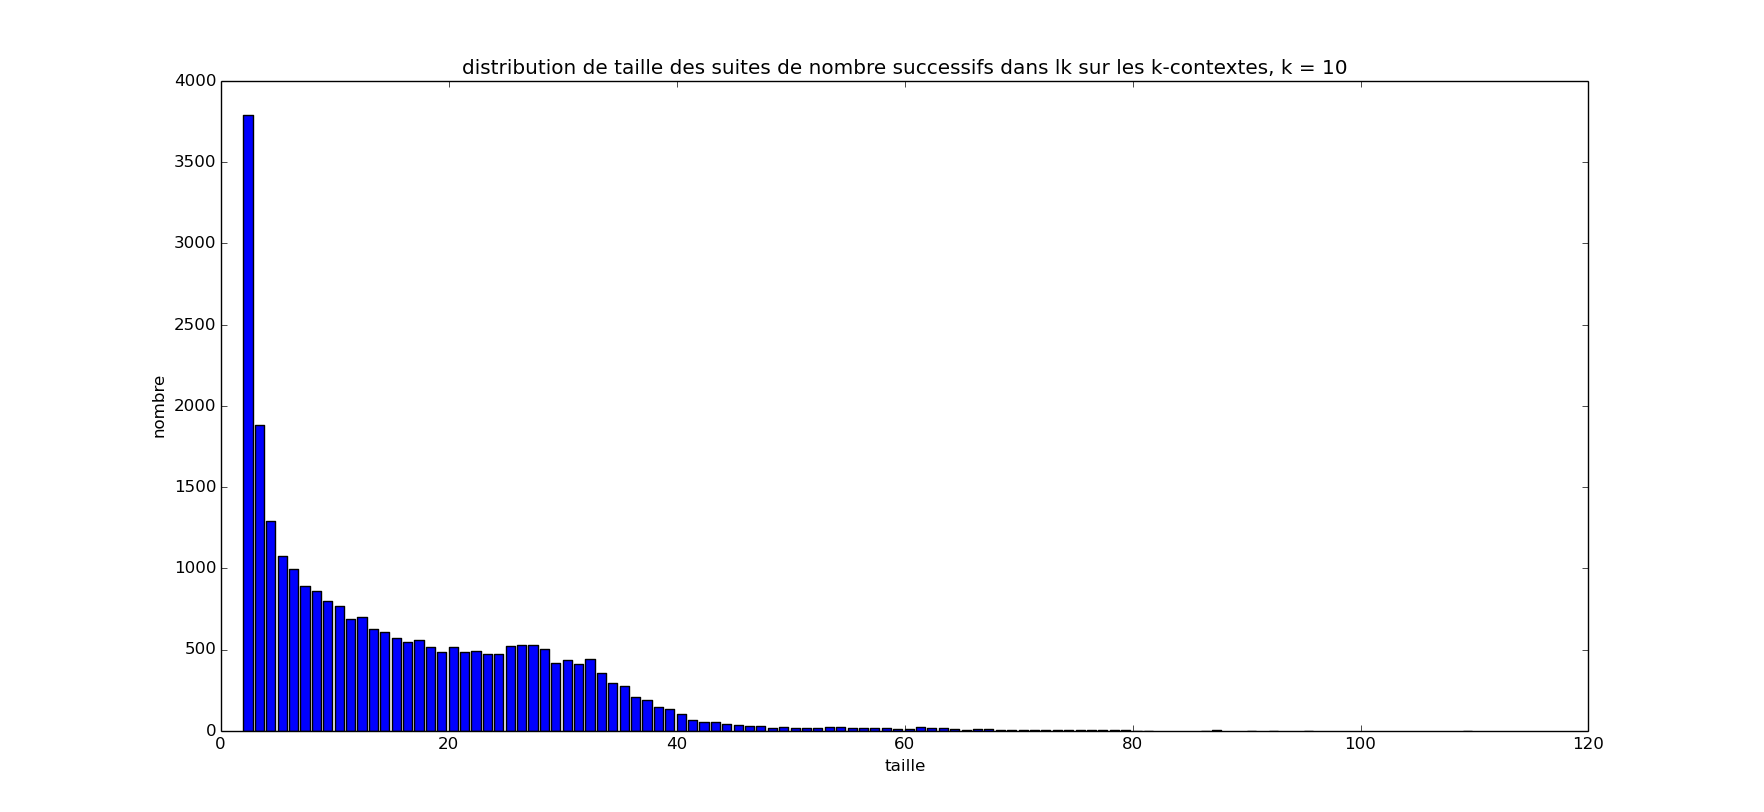
\includegraphics[scale = 0.3]{./images/suitesLFreads10K_k10.png}
    \caption{Reads10K est un ensemble de 500 reads de taille 70. On s'aperçoit qu'il y a plus de 7000 suites de nombres successifs supérieures à 20.}
    \label{suitesLF}
\end{figure}

La deuxième approche consiste à regarder la différence entre la fonction LF() et $LF'(i) = C[i] + rank(\bwt[i], i)$, à savoir la fonction utilisée pour calculer LF() sur la \bwt.




%%%%%%%% chevauchement de reads dans les k-contextes





%
%Premières idées :
%	. chercher par blocs (-> seulement quand bloc assez grand)
%	. stocker permutations (-> infos ne peut pas se contenir elle meme ; décrire différentes idées stockage)

%Implémentation pour tester faisabilité         |  
%étude de la compression                        | -> dans Résultats ?
%calcul de l'entropie pour voir si correspond   | 
%compression avec compresseurs existants        |
%
%pour recherche, besoin de lf. pour lf besoin struc Petri -> lourd
%sur k-contextes, lf croissante -> stocker lf ? mieux
%
%lf lourde
%essais compression
%
%petits k-contextes qd \$ dans contexte -> enlever ces contextes ?
%non

\subsection{Résultats} 

\begin{figure}[!ht]
    \center
    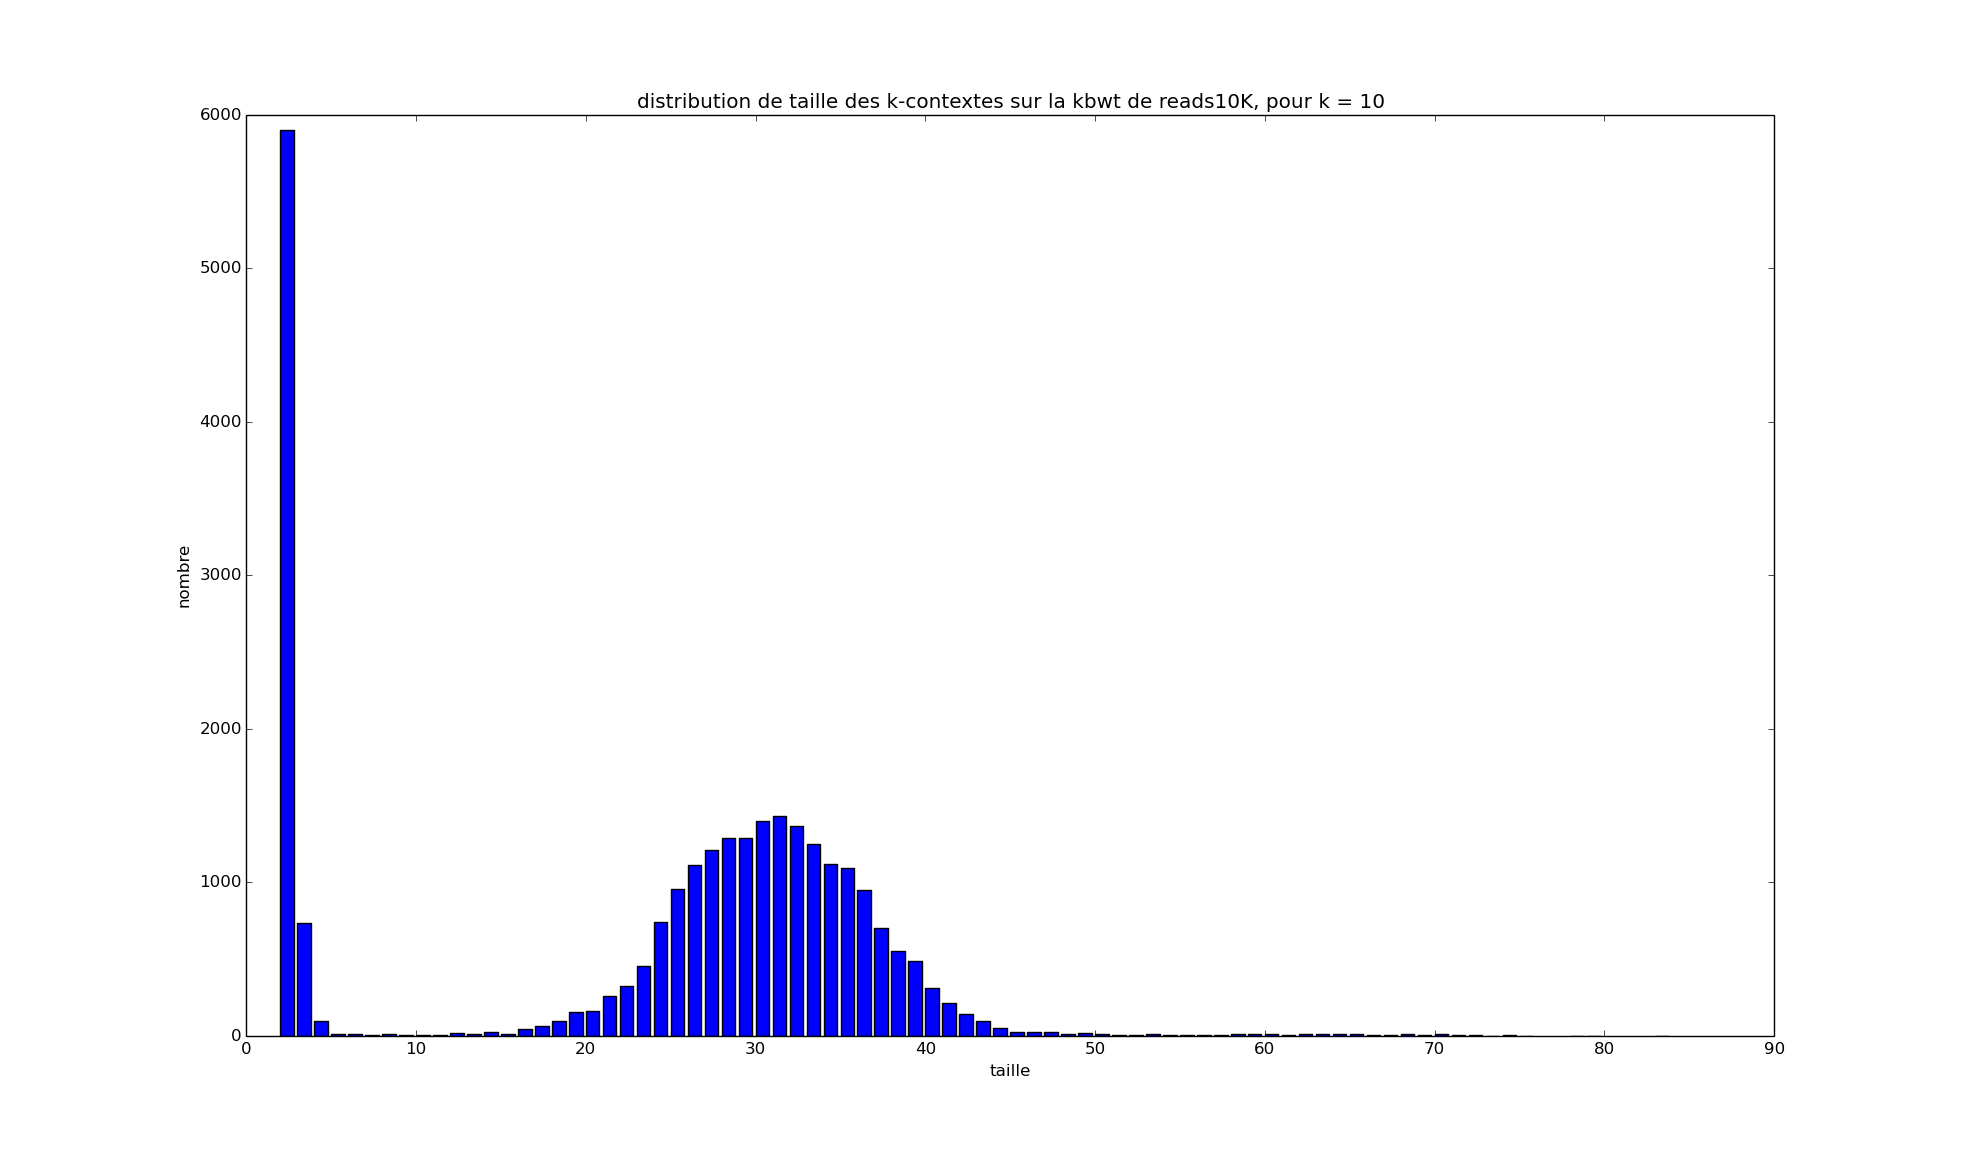
\includegraphics[scale=0.3]{./images/distribReads10K_k10.png}
    \caption{Reads10K est un ensemble de 500 reads de taille 70. On peut voir que la \kbwt\ triée de cet ensemble comprend environ 15 000 $k$-contextes de taille entre 25 et 40. Les presque 6000 $k$-contextes de taille 2 correspondent aux $k$-contextes chevauchant deux reads.}
    \label{chromato}
\end{figure}

expliquer les stuctures et algos les plus efficaces et donner les temps d'accès et taux de compression.
